%% Submissions for peer-review must enable line-numbering
%% using the lineno option in the \documentclass command.
%%
%% Preprints and camera-ready submissions do not need
%% line numbers, and should have this option removed.
%%
%% Please note that the line numbering option requires
%% version 1.1 or newer of the wlpeerj.cls file, and
%% the corresponding author info requires v1.2

\documentclass[fleqn,10pt,lineno]{wlpeerj} % for journal submissions

% ZNK -- Adding headers for pandoc

\setlength{\emergencystretch}{3em}
\usepackage[unicode=true]{hyperref}


% tightlist command for lists without linebreak
\providecommand{\tightlist}{%
  \setlength{\itemsep}{0pt}\setlength{\parskip}{0pt}}

% From pandoc table feature
\usepackage{longtable,booktabs,array}
\usepackage{calc} % for calculating minipage widths
% Correct order of tables after \paragraph or \subparagraph
\usepackage{etoolbox}
\makeatletter
\patchcmd\longtable{\par}{\if@noskipsec\mbox{}\fi\par}{}{}
\makeatother
% Allow footnotes in longtable head/foot
\IfFileExists{footnotehyper.sty}{\usepackage{footnotehyper}}{\usepackage{footnote}}
\makesavenoteenv{longtable}

% Pandoc citation processing
%From Pandoc 3.1.8
% definitions for citeproc citations
\NewDocumentCommand\citeproctext{}{}
\NewDocumentCommand\citeproc{mm}{%
  \begingroup\def\citeproctext{#2}\cite{#1}\endgroup}
\makeatletter
 % allow citations to break across lines
 \let\@cite@ofmt\@firstofone
 % avoid brackets around text for \cite:
 \def\@biblabel#1{}
 \def\@cite#1#2{{#1\if@tempswa , #2\fi}}
\makeatother
\newlength{\cslhangindent}
\setlength{\cslhangindent}{1.5em}
\newlength{\csllabelwidth}
\setlength{\csllabelwidth}{3em}
\newenvironment{CSLReferences}[2] % #1 hanging-indent, #2 entry-spacing
 {\begin{list}{}{%
  \setlength{\itemindent}{0pt}
  \setlength{\leftmargin}{0pt}
  \setlength{\parsep}{0pt}
  % turn on hanging indent if param 1 is 1
  \ifodd #1
   \setlength{\leftmargin}{\cslhangindent}
   \setlength{\itemindent}{-1\cslhangindent}
  \fi
  % set entry spacing
  \setlength{\itemsep}{#2\baselineskip}}}
 {\end{list}}
\usepackage{calc}
\newcommand{\CSLBlock}[1]{#1\hfill\break}
\newcommand{\CSLLeftMargin}[1]{\parbox[t]{\csllabelwidth}{#1}}
\newcommand{\CSLRightInline}[1]{\parbox[t]{\linewidth - \csllabelwidth}{#1}\break}
\newcommand{\CSLIndent}[1]{\hspace{\cslhangindent}#1}

\usepackage{fancyhdr}
\pagestyle{fancy}
\fancyhead[L]{Harmon \& Revell (2025)}
\fancyhead[C]{}
\fancyhead[R]{Semi-parametric comparative method}
\usepackage[singlelinecheck=false]{caption}
\usepackage{amsmath,mathtools,bm}


\title{A Semiparametric Method to Test for Correlated Evolution in a Phylogenetic Context}

\author[1]{Luke J. Harmon}

\corrauthor[1]{Luke J. Harmon}{\href{mailto:lukeh@uidaho.edu}{\nolinkurl{lukeh@uidaho.edu}}}
\author[2]{Liam J. Revell}


\affil[1]{Department of Biological Sciences, University of Idaho, Moscow, ID, USA}
\affil[2]{Department of Biology, University of Massachusetts Boston, Boston, MA, USA}


%
% \author[1]{First Author}
% \author[2]{Second Author}
% \affil[1]{Address of first author}
% \affil[2]{Address of second author}
% \corrauthor[1]{First Author}{f.author@email.com}

% 

\begin{abstract}
Phylogenetic comparative methods are a broad suite of approaches for studying trait and species diversification using evolutionary trees. In spite of their extraordinary growth in sophistication and complexity in recent years, among the most commonly-employed phylogenetic comparative method is the simple measure of the evolutionary correlation between variables, whilst accounting for the statistical non-independence that arises from common descent. The standard parametric approach for measuring the evolutionary correlation of continuously-valued characters on a phylogeny assumes a model called Brownian motion for the evolution of our traits. Here, we introduce a new semi-parametric method that relaxes this assumption by testing for the evolutionary correlation between variables based on ranks, and then obtaining a null distribution on the test statistic via random permutation. We show that this approach has reasonable statistical properties: type I error close to the nominal level, and power that is similar to fully parametric methods. We conclude by comparing our new method to related approaches.
% Dummy abstract text. Dummy abstract text. Dummy abstract text. Dummy abstract text. Dummy abstract text. Dummy abstract text. Dummy abstract text. Dummy abstract text. Dummy abstract text. Dummy abstract text. Dummy abstract text.
\end{abstract}

\begin{document}



\flushbottom
\maketitle
\thispagestyle{empty}

\section{Introduction}\label{introduction}

Statistical phylogenetic comparative methods have become an invaluable tool in contemporary evolutionary research (Felsenstein 1985; Revell and Harmon 2022). This set of methodologies comprises a large and growing set of approaches for studying increasingly sophisticated evolutionary hypotheses of trait and species diversification using phylogenies (reviewed in Harvey and Pagel 1991; Nunn 2011; O'Meara 2012; Harmon 2019; Revell and Harmon 2022). Nonetheless, among the most common evolutionary hypothesis studied by researchers is the simple question of whether one trait is correlated with another, while accounting for the statistical non-independence of the species that that make up our data points due to their shared histories (Felsenstein 1985; reviewed in Harmon 2019; Revell and Harmon 2022).

When measuring and undertaking a hypothesis test of this correlation, phylogenetic comparative methods must typically assume a particular underlying model of trait evolution, such as the Brownian motion model (Felsenstein 1973; Felsenstein 1985; O'Meara et al. 2006). In particular, under the algorithm of phylogenetically independent contrasts, both the internal node values in the contrasts algorithm, and the variances of the (non-standardized) contrasts are calculated assuming a Brownian evolutionary process on the tree (Felsenstein 1985; Harmon 2019). Likewise, under phylogenetic generalized least squares regression (Grafen 1989), we assume that either the data themselves or their residual error are autocorrelated in a manner consistent with Brownian motion evolution or a close relative (e.g., Pagel 1999; Garland and Ives 2000; Rohlf 2001; Revell 2010). Although there are some circumstances under which continuously-valued phenotypic traits might genuinely evolve via a Brownian process (e.g., Lynch 1990), violations of the Brownian model are likely be common in real data sets (Freckleton and Harvey 2006; Hunt 2006; Estes and Arnold 2007; Uyeda et al. 2011). The Brownian motion model has nonetheless persisted as one of the most commonly-used trait evolution models in studying evolutionary correlations, largely due to its simplicity, tractability, and apparent robustness to deviations from model assumptions under some circumstances (e.g., Garland et al. 1993; Stone 2011).

A number of approaches have been devised to identify violations of Brownian motion in our data in measuring the evolutionary correlation, and then to account for these deviations statistically. First, one can apply various diagnostic tests for independent contrasts that are sensitive to a variety of violations of the Brownian model (Garland 1992; Blomberg et al. 2003; Freckleton and Harvey 2006). For example, if the true model is Brownian motion, then standardized independent contrasts of Felsenstein (1985) should be independently and identically distributed (i.i.d.). If, on the other hand, standardized contrasts are correlated with their expected variance (the amount of evolutionary branch length that subtends the contrast), this suggests that there is more or less change along long branches of the tree (depending on the sign of the correlation) than expected under Brownian motion. One can then attempt various transformations of the branch lengths of the tree so that the contrasts no longer violate our test (Garland 1992). Another similar diagnostic is the node-height test, in which we test for a relationship between the standardized contrasts and the height of the node over which they are calculated (Freckleton and Harvey 2006). Once again, this correlation should be absent if the Brownian motion model assumptions hold. In both instances, one can consider these tests to be measurements of model adequacy, where failure of the test suggests that the underlying assumption of Brownian motion could be invalid (Pennell et al. 2015).

Under circumstances in which the Brownian motion assumption is violated, one can always consider alternative models (e.g., Pagel 1999). In phylogenetic comparative methods,however, our alternative models are typically limited to a few simple alternatives. One can attempt, for example, different evolutionary models that are nonetheless Gaussian, such as the Ornstein-Uhlenbeck or a speciational trait evolution models (e.g., Hansen 1997; Martins and Hansen 1997). Likewise, one can transform the branches of the phylogenetic tree or the elements of the variance-covariance matrix derived from the tree (Grafen 1989; Garland 1992; Pagel 1999). Nonetheless, there is no general solution and on occasion there may be no way to coax certain data sets to fit the particular assumptions of our analyses.

In statistics, nonparametric tests can sometimes provide robustness in cases where models are not known or provide poor fits to data (e.g., Wasserman 2006). As comparative methods are employed to tackle a wider and wider range of problems, from genomics to cancer biology to evolutionary studies at the broadest scale, there is a growing need for methods that are robust to model violations. Among existing comparative methods, there are nonparametric methods available for the analysis of discrete characters (e.g., Maddison 1990) and morphometric shape data (Adams 2014). To date, however, the only available nonparametric comparative method designed specifically for continuously distributed trait data is Ackerly's (2000) contrast sign test (CST). This test compares the signs (positive or negative) of phylogenetically independent contrasts for two characters. If the two characters are evolving independently, then the number of pairs of contrasts with the same sign should follow a binomial distribution with probability of success p=0.5. This test provides a robust alternative to parametric comparative methods, but is not commonly used. The main drawback of Ackerly's approach is that it has low power, partially because it uses only the signs, and not the magnitudes, of the contrasts.

Here we describe a new semiparametric comparative method, the phylogenetic rank correlation (PRC) test.

This test, which is based on the correlation of ranks of independent contrasts on a phylogenetic tree, is robust under several models of trait evolution, and has power comparable to standard independent contrasts and much greater than the CST. We argue that the PRC test thus may provide a robust alternative to parametric methods such as PGLS and independent contrasts.

\section{Description of the Method}\label{description-of-the-method}

The PRC test has six steps (Figure 1):

\begin{enumerate}
\def\labelenumi{\arabic{enumi}.}
\item
  Calculate standardized independent contrasts (Felsenstein 1985) for two continuously distributed traits.
\item
  Reflect the contrasts, multiplying both the \(X\) and \(Y\) value of each contrast by \(-1\). The data will now include two `copies' of each contrast, one with the signs of each contrast reversed.
\item
  Create ranks independently for each variable. For tied scores, assign the mean rank to all tied contrasts.
\item
  Calculate the test statistic. Here, we use Spearman's rank correlation coefficient, but one could also use Kendall's \(\tau\).
\item
  Generate the null distribution of the test statistic via randomization of the contrasts. To do this, permute the independent contrasts for one variable. Then, create new ranks, and calculate the test statistic. Repeat this permutation procedure a large number of times (say, 9,999) to generate a null distribution. (We can either permute the doubled contrasts or permute the original contrasts and double them -- the result will be the same.)
\item
  Compare the test statistic with the null distribution from permutation to obtain a P-value of the test.
\end{enumerate}

\begin{figure}
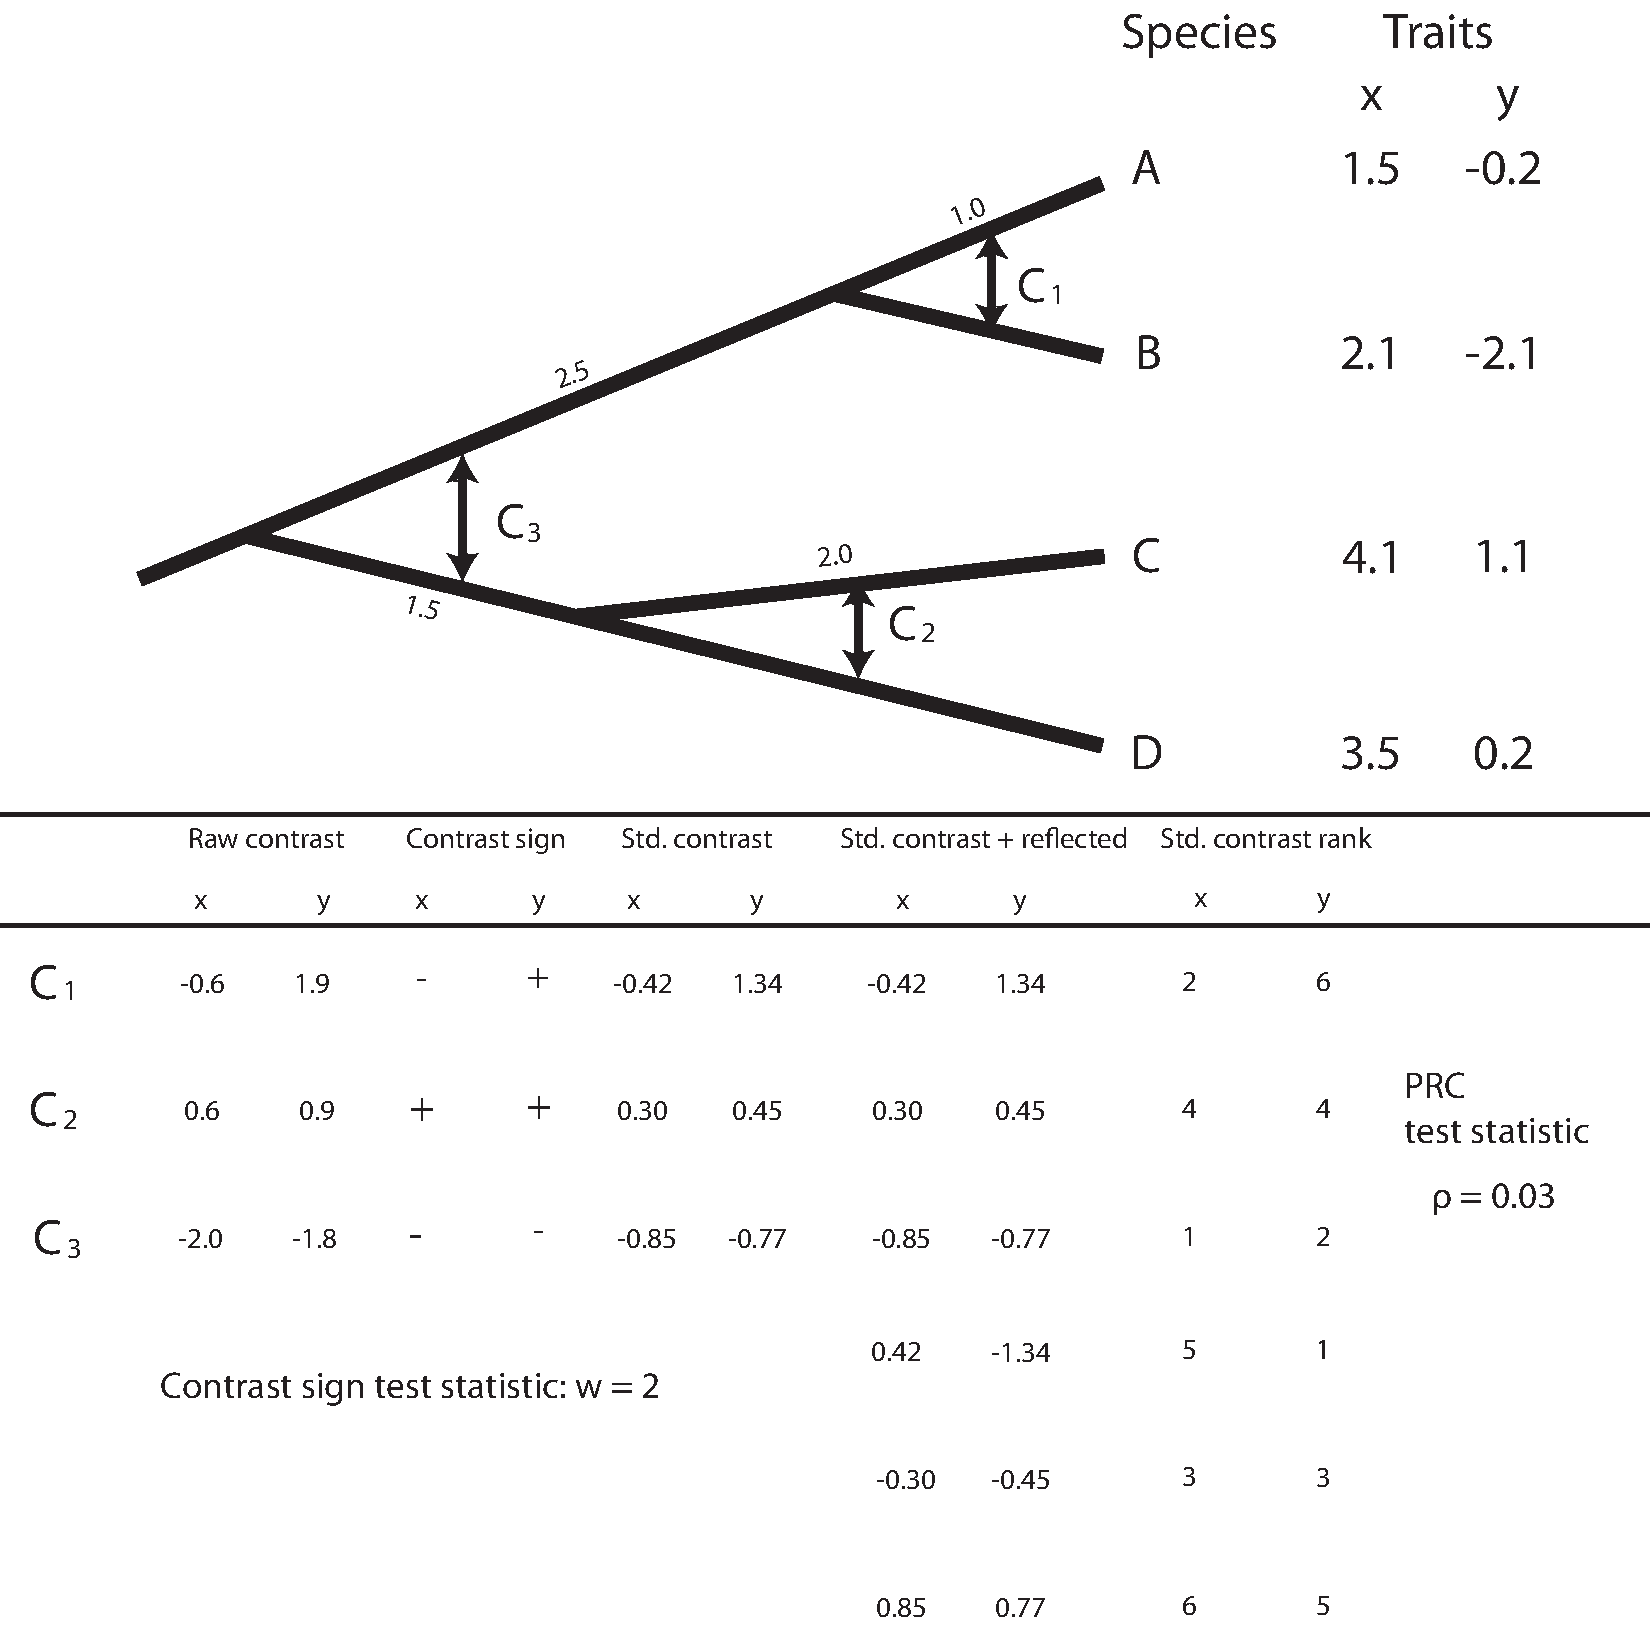
\includegraphics[width=1\linewidth]{schematic} \caption{Illustration of the method of phylogenetic rank contrasts, PRC. First, compute the raw contrasts. For a bifurcation tree with $N$ tips there should be $N-1$ such contrasts. Next, standardize the contrasts by their expected variance in the typical way following Felsenstein (1985). Duplicate all pairs of contrasts for each of our two variable but swapping the signs. Convert all contrasts (and their reflections) to ranks. Calculate the test-statistic. See main text for more details.}\label{fig:Harmon-fig1}
\end{figure}

Several of these steps require additional comments or explanations.

For step one, standardized contrasts are calculated. The calculation of these contrasts, as originally described by Felsenstein (1985), assumes a Brownian motion model of evolution; however, since the standardized contrasts are converted into ranks, violating this assumption has little effect on the analysis (see below). In practice, by converting contrasts into ranks, we assume only that contrasts subtending longer branches of the tree tend to be larger in absolute magnitude. This assumption is compatible with a wide range of evolutionary models as long as variance among species tends to increase through time (see Estes and Arnold 2007).

Reflecting the contrasts (step 2) is necessary because the direction of any particular contrast is arbitrary. Reflecting contrasts across the axes ensures that the analysis is unchanged by rotating the nodes in the tree. This procedure is the statistical equivalent of forcing the regression through the origin, which is required when testing for correlations of independent contrasts (Garland et al. 1992). We do not have to worry about inflating degrees of freedom by doubling the number of data points because statistical significance is to be determined by permutations.

Finally, in step 4, any nonparametric test statistic could be used for this test (see, e.g., Wasserman 2006). We used Spearman's rank correlation, which is simply the Pearson product-moment correlation of the ranks of the two variables. Kendall's \(\tau\) is another viable option.

We provide a worked example of the calculations involved in this test in Figure 2. Software to carry out this test, written in the R statistical computing language (R Core Team 2024) and will be made publicly available as part of the GEIGER R package (Harmon et al. 2007; Pennell et al. 2014)

\section{Statistical properties of the method}\label{statistical-properties-of-the-method}

We compared the statistical performance of the PRC method with both non-phylogenetic (standard regression) and phylogenetic comparative methods (independent contrasts, IC, and the contrast sign test, CST; see Fig. 2 legend for simulation details). Like independent contrasts and the contrast sign test, the PRC test has appropriate type-I error under a Brownian motion model (Fig. 2a). However, both alternative tests outperform both standard correlation tests and independent contrasts when models of evolution are non-Brownian (Fig. 2b). Independent contrasts fail when there is little phylogenetic structure in the data, as under an Ornstein-Uhlenbeck model with a high \(\alpha\) parameter (Fig. 2b). Similarly, standard correlation fails when data has a strong phylogenetic component, as under Brownian motion (Fig. 2b). Both alternative methods have type I error near 5/\% under a range of \(\alpha\) values. Type I error rates for the rank test are only slightly elevated (7/\%) compared to its nominal level.

\begin{figure}
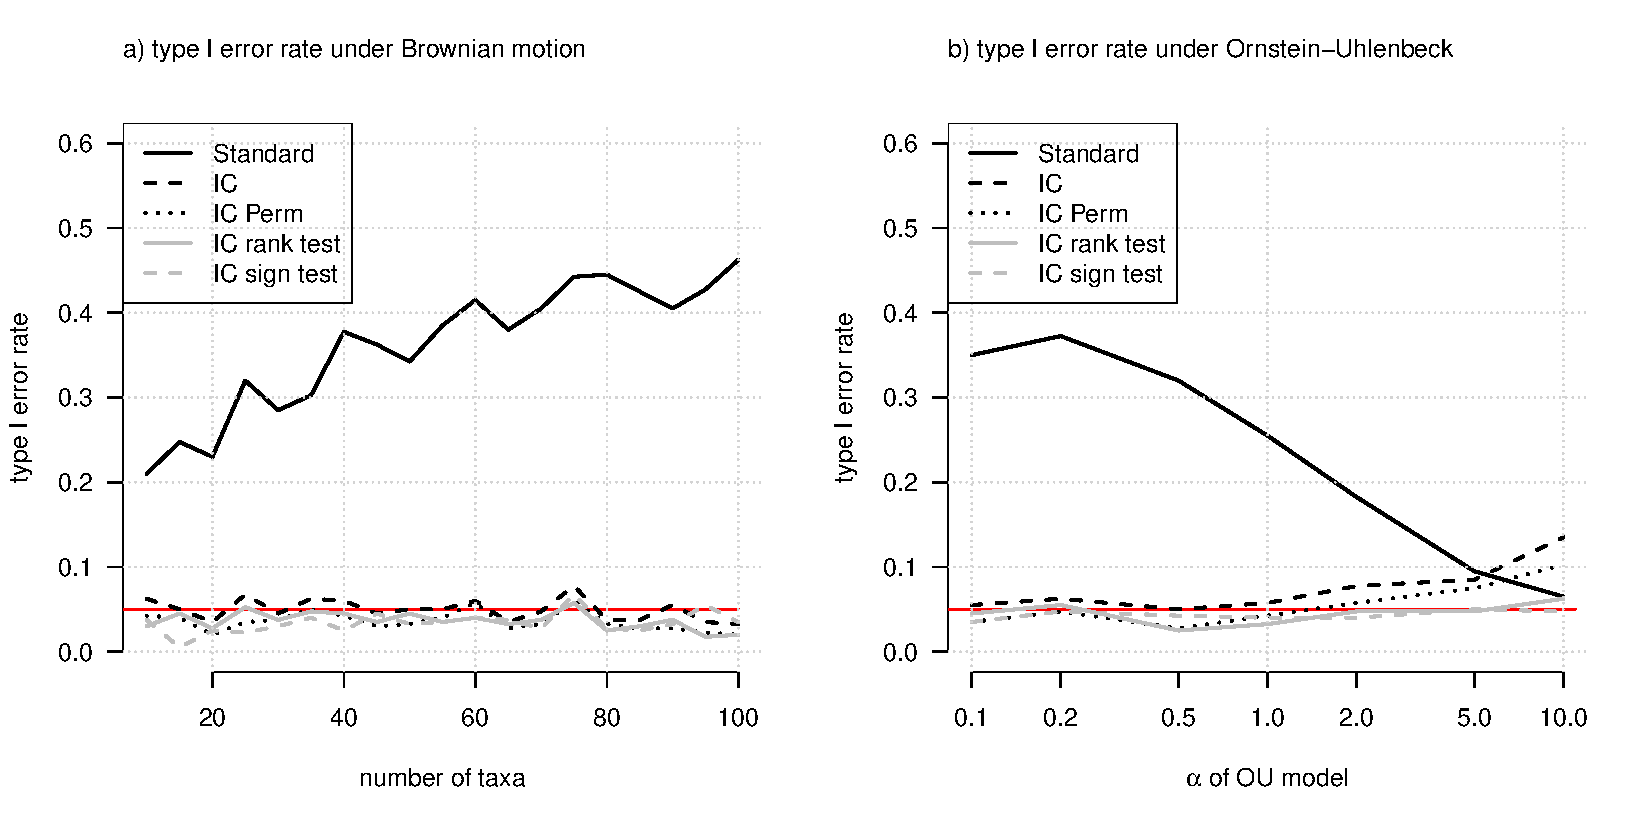
\includegraphics[width=1\linewidth]{Harmon-and-Revell_NonParametricPCM.PeerJ_files/figure-latex/Harmon-fig2-1} \caption{Type I error results.}\label{fig:Harmon-fig2}
\end{figure}

Likewise, our PRC method has only slightly less power than standard independent contrasts, and considerably more power than Ackerly's (2000) sign test, over both a range of tree sizes and character correlation values (Fig. 3a, b). The PRC test also outperforms other comparative methods when there is error in phylogenetic branch length estimation. To illustrate this, we simulated data on pure-birth phylogenetic trees (as in Figure 1) but then ran analyses after setting all branch lengths in these trees equal. Under these conditions, both PRC and the contrast sign test have appropriate type I error (CST 2.0/\%, PRC 5.7/\%), while type I error is elevated for independent contrasts (11.4/\%). When the expected correlation between characters is 0.5, PRC again has power similar to independent contrasts (IC 74.6/\%, PRC 62.9/\%). This test also mimics the situation where one knows tree topology, but branch lengths are either unknown or estimated with high error.

\begin{figure}
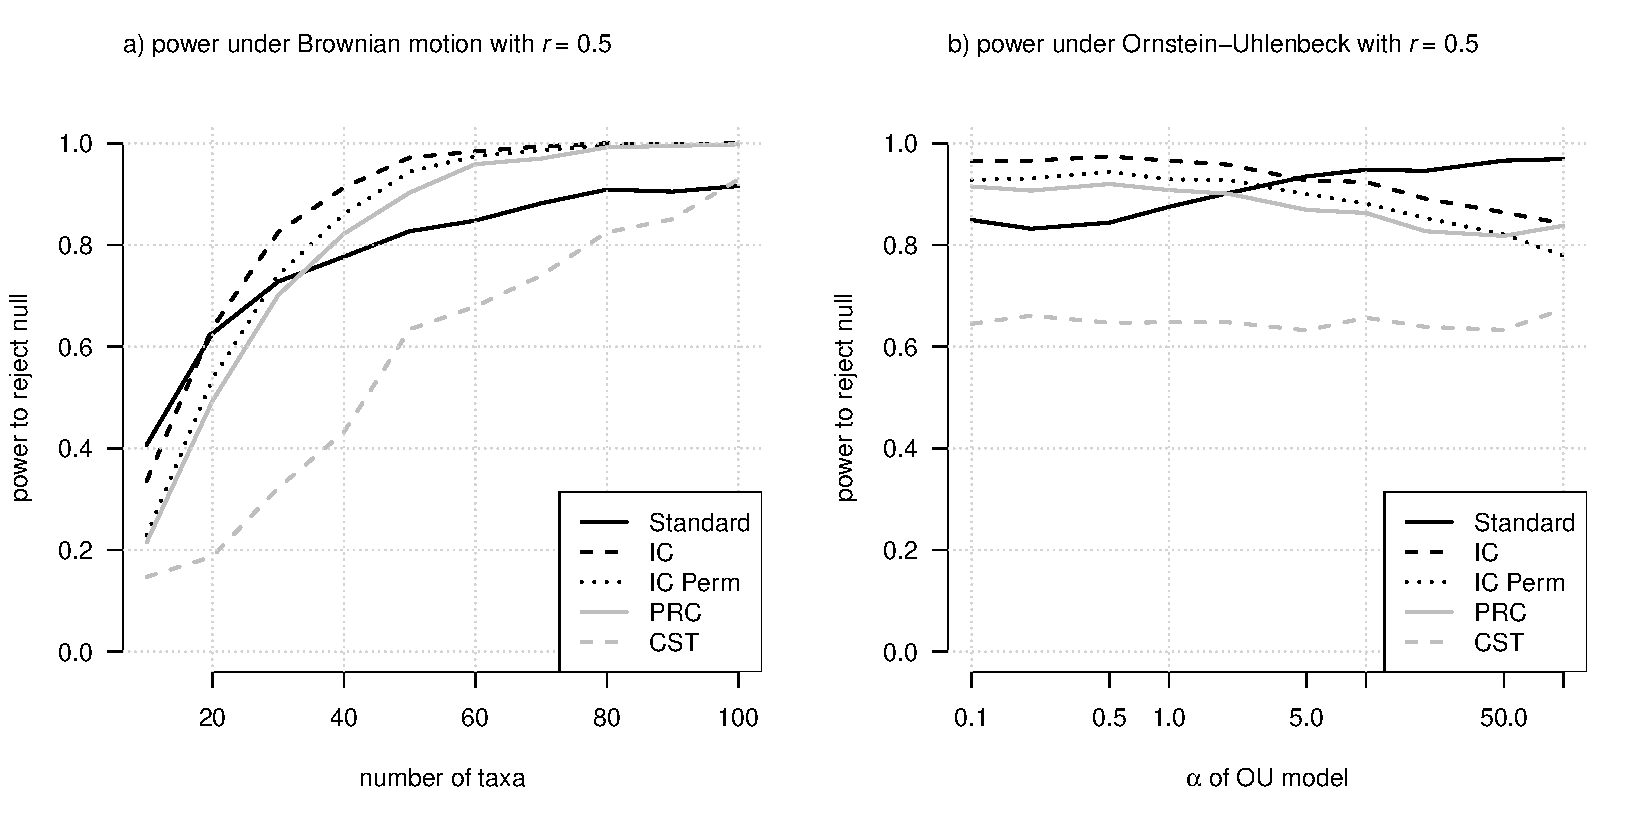
\includegraphics[width=1\linewidth]{Harmon-and-Revell_NonParametricPCM.PeerJ_files/figure-latex/Harmon-fig3-1} \caption{Power analysis results.}\label{fig:Harmon-fig3}
\end{figure}

We have characterized this method as ``semiparametric'' because it is not truly distribution-free. One key component of the method involves calculating standardized independent contrasts, which assumes that the characters are evolving under a Brownian motion model. However, by converting these contrasts to ranks, this method greatly lessens the effects of violations of this assumption for testing correlations between characters. In fact, to preserve contrast rank order, one must assume that changes on each branch are independent, and that there is more change on longer branches in the tree than along short branches. Violations of this assumption will lead to increased type I error of this test. One example of violations that would have negative impacts on all tests described here (standard regression, independent contrasts, CST, and PST) is rate heterogeneity across the tree (O'Meara et al., 2006). For example, if evolution is faster along certain branches in the tree, nearby contrasts values and signs will be correlated, and all methods relying on their independence will exhibit inflated type I error.

Table 1 shows a summary of our results. (Should we need to include a table, I'm leaving this in as a guide for formatting it.)

\begin{table}

\caption{\label{tab:unnamed-chunk-6}Example table. See main text for more details.}
\centering
\begin{tabular}[t]{l|l|l|l|l|l}
\hline
  & log(L) & estimated $\alpha$ & d.f. & AIC & weight\\
\hline
directional one-rate M\emph{k} & -- & -- & -- & -- & --\\
\hline
ordered two-rate M\emph{k} & -- & -- & -- & -- & --\\
\hline
ordered ten-rate M\emph{k} & -- & -- & -- & -- & --\\
\hline
\end{tabular}
\end{table}

\section{Conclusions}\label{conclusions}

Since the model of evolution underlying continuous characters is frequently unknown, and may depart from Brownian motion,we recommend using this method to test correlations between characters. If standard contrasts are well-behaved, then standard techniques are still useful for estimating slopes and other parameter values. However, this semiparametric test provides a method for generating robust P-values across a range of models. The technique is nearly as powerful as independent contrasts but much more robust to deviations from the underlying model of evolution.

\section{Data availability}\label{data-availability}

This article was written in Rmarkdown (Xie et al. 2018, 2020; Allaire et al. 2023), and developed with the help of both \emph{bookdown} (Xie 2016, 2023) and the posit Rstudio IDE (RStudio Team 2020). All data and markdown code necessary to exactly rebuild the submitted version of this article (including its analyses and figures) are available at \url{https://github.com/liamrevell/Revell-and-Harmon.NonParametricPCM}.

\section{Acknowledgments}\label{acknowledgments}

We thank J. J. Kolbe, J. B. Losos, D. Schluter, R. E. Glor, B. Banbury, T. Hagey, C. Brock, and H. Alamillo for providing helpful feedback on this paper.

\section*{Literature Cited}\label{literature-cited}
\addcontentsline{toc}{section}{Literature Cited}

\phantomsection\label{refs}
\begin{CSLReferences}{1}{0}
\bibitem[\citeproctext]{ref-Ackerly2000}
Ackerly, D. D. 2000. \href{https://doi.org/10.1111/j.0014-3820.2000.tb00694.x}{TAXON SAMPLING, CORRELATED EVOLUTION, AND INDEPENDENT CONTRASTS}. Evolution 54:1480--1492. Wiley.

\bibitem[\citeproctext]{ref-Adams2014}
Adams, D. C. 2014. A method for assessing phylogenetic least squares models for shape and other high-dimensional multivariate data. Evolution 68:2675--2688. Wiley.

\bibitem[\citeproctext]{ref-Allaire2023}
Allaire, J., Y. Xie, J. McPherson, J. Luraschi, K. Ushey, A. Atkins, H. Wickham, J. Cheng, W. Chang, and R. Iannone. 2023. \href{https://github.com/rstudio/rmarkdown}{{R}markdown: Dynamic documents for {R}}.

\bibitem[\citeproctext]{ref-Blomberg2003}
Blomberg, S. P., T. Garland, and A. R. Ives. 2003. \href{https://doi.org/10.1111/j.0014-3820.2003.tb00285.x}{Testing for phylogenetic signal in comparative data: Behavioral traits are more labile}. Evolution 57:717--745. Wiley.

\bibitem[\citeproctext]{ref-Estes2007}
Estes, S., and S. J. Arnold. 2007. Resolving the paradox of stasis: Models with stabilizing selection explain evolutionary divergence on all timescales. Am. Nat. 169:227--244.

\bibitem[\citeproctext]{ref-Felsenstein1973a}
Felsenstein, J. 1973. Maximum-likelihood estimation of evolutionary trees from continuous characters. American Journal of Human Genetics 25:471--492.

\bibitem[\citeproctext]{ref-Felsenstein1985}
Felsenstein, J. 1985. Phylogenies and the comparative method. Am. Nat. 125:1--15.

\bibitem[\citeproctext]{ref-Freckleton2006}
Freckleton, R. P., and P. H. Harvey. 2006. Detecting non-brownian trait evolution in adaptive radiations. PLoS Biol. 4:e373. Public Library of Science (PLoS).

\bibitem[\citeproctext]{ref-Garland2000}
Garland, Jr., and A. R. Ives. 2000. Using the past to predict the present: Confidence intervals for regression equations in phylogenetic comparative methods. Am. Nat. 155:346--364. University of Chicago Press.

\bibitem[\citeproctext]{ref-Garland1992}
Garland, T., Jr. 1992. Rate tests for phenotypic evolution using phylogenetically independent contrasts. Am. Nat. 140:509--519.

\bibitem[\citeproctext]{ref-Garland1993}
Garland, T., A. W. Dickerman, C. M. Janis, and J. A. Jones. 1993. Phylogenetic analysis of covariance by computer simulation. Syst. Biol. 42:265--292. Oxford Academic.

\bibitem[\citeproctext]{ref-Garland1992b}
Garland, T., P. H. Harvey, and A. R. Ives. 1992. \href{https://doi.org/10.1093/sysbio/41.1.18}{Procedures for the analysis of comparative data using phylogenetically independent contrasts}. Systematic Biology 41:18--32. Oxford University Press (OUP).

\bibitem[\citeproctext]{ref-Grafen1989}
\href{https://doi.org/10.1098/rstb.1989.0106}{Grafen, A. 1989. Philosophical Transactions of the Royal Society of London. B, Biological Sciences 326:119--157. The Royal Society}.

\bibitem[\citeproctext]{ref-Hansen1997}
Hansen, T. F. 1997. \href{https://doi.org/10.1111/j.1558-5646.1997.tb01457.x}{STABILIZING SELECTION AND THE COMPARATIVE ANALYSIS OF ADAPTATION}. Evolution 51:1341--1351. Wiley.

\bibitem[\citeproctext]{ref-Harmon2019-book}
Harmon, L. J. 2019. Phylogenetic comparative methods: Learning from trees. Ecoevorxiv.

\bibitem[\citeproctext]{ref-Harmon2007}
Harmon, L. J., J. T. Weir, C. D. Brock, R. E. Glor, and W. Challenger. 2007. \href{https://doi.org/10.1093/bioinformatics/btm538}{GEIGER: Investigating evolutionary radiations}. Bioinformatics 24:129--131. Oxford University Press (OUP).

\bibitem[\citeproctext]{ref-Harvey1991}
Harvey, P. H., and M. D. Pagel. 1991. The comparative method in evolutionary biology. Oxford University Press, Oxford, UK.

\bibitem[\citeproctext]{ref-Hunt2006}
Hunt, G. 2006. Fitting and comparing models of phyletic evolution: Random walks and beyond. Paleobiology 32:578--601. The Paleontological Society.

\bibitem[\citeproctext]{ref-Lynch1990}
Lynch, M. 1990. The rate of morphological evolution in mammals from the standpoint of the neutral expectation. Am. Nat. 136:727--741.

\bibitem[\citeproctext]{ref-Maddison1990}
Maddison, W. P. 1990. \href{https://doi.org/10.2307/2409435}{A method for testing the correlated evolution of two binary characters: Are gains or losses concentrated on certain branches of a phylogenetic tree?} Evolution 44:539--557. Society for the Study of Evolution.

\bibitem[\citeproctext]{ref-Martins1997}
Martins, E. P., and T. F. Hansen. 1997. \href{https://doi.org/10.1086/286013}{Phylogenies and the comparative method: A general approach to incorporating phylogenetic information into the analysis of interspecific data}. The American Naturalist 149:646--667. University of Chicago Press.

\bibitem[\citeproctext]{ref-Nunn2011-book}
Nunn, C. L. 2011. The comparative approach in evolutionary anthropology and biology. University of Chicago Press.

\bibitem[\citeproctext]{ref-OMeara2012}
O'Meara, B. C. 2012. \href{https://doi.org/10.1146/annurev-ecolsys-110411-160331}{Evolutionary inferences from phylogenies: A review of methods}. Annual Review of Ecology, Evolution, and Systematics 43:267--285. Annual Reviews.

\bibitem[\citeproctext]{ref-OMeara2006}
O'Meara, B. C., C. Ané, M. J. Sanderson, and P. C. Wainwright. 2006. \href{https://doi.org/10.1111/j.0014-3820.2006.tb01171.x}{Testing for different rates of continuous trait evolution using likelihood}. Evolution 60:922--933. Wiley.

\bibitem[\citeproctext]{ref-Pagel1999}
Pagel, M. 1999. \href{https://doi.org/10.1080/106351599260184}{The maximum likelihood approach to reconstructing ancestral character states of discrete characters on phylogenies}. Systematic Biology 48:612--622. Oxford University Press (OUP).

\bibitem[\citeproctext]{ref-Pennell2014}
Pennell, M. W., J. M. Eastman, G. J. Slater, J. W. Brown, J. C. Uyeda, R. G. FitzJohn, M. E. Alfaro, and L. J. Harmon. 2014. \href{https://doi.org/10.1093/bioinformatics/btu181}{Geiger v2.0: An expanded suite of methods for fitting macroevolutionary models to phylogenetic trees}. Bioinformatics 30:2216--2218. Oxford University Press (OUP).

\bibitem[\citeproctext]{ref-Pennell2015}
Pennell, M. W., R. G. FitzJohn, W. K. Cornwell, and L. J. Harmon. 2015. Model adequacy and the macroevolution of angiosperm functional traits. Am. Nat. 186:E33--E50. University of Chicago Press Chicago, IL.

\bibitem[\citeproctext]{ref-RCoreTeam2024}
R Core Team. 2024. \href{https://www.R-project.org/}{R: A language and environment for statistical computing}. R Foundation for Statistical Computing, Vienna, Austria.

\bibitem[\citeproctext]{ref-Revell2010}
Revell, L. J. 2010. Phylogenetic signal and linear regression on species data. Methods Ecol. Evol. 1:319--329. Wiley.

\bibitem[\citeproctext]{ref-Revell2022-book}
Revell, L. J., and L. J. Harmon. 2022. Phylogenetic comparative methods in {R}. Princeton University Press, Princeton, NJ.

\bibitem[\citeproctext]{ref-Rohlf2001}
Rohlf, F. J. 2001. \href{https://doi.org/10.1111/j.0014-3820.2001.tb00731.x}{Comparative methods for the analysis of continuous variables: Geometric interpretations}. Evolution 55:2143--2160. Wiley.

\bibitem[\citeproctext]{ref-Rstudio2020}
RStudio Team. 2020. \href{http://www.rstudio.com/}{R{S}tudio: Integrated development environment for {R}}. RStudio, PBC., Boston, MA.

\bibitem[\citeproctext]{ref-Stone2011}
Stone, E. A. 2011. \href{https://doi.org/10.1093/sysbio/syq098}{Why the phylogenetic regression appears robust to tree misspecification}. Systematic Biology 60:245--260. Oxford University Press (OUP).

\bibitem[\citeproctext]{ref-Uyeda2011}
Uyeda, J. C., T. F. Hansen, S. J. Arnold, and J. Pienaar. 2011. The million-year wait for macroevolutionary bursts. Proc. Natl. Acad. Sci. U. S. A. 108:15908--15913.

\bibitem[\citeproctext]{ref-Wasserman2006}
Wasserman, L. 2006. \href{https://doi.org/10.1007/0-387-30623-4}{All of nonparametric statistics}. Springer Science \& Business Media, New York, NY.

\bibitem[\citeproctext]{ref-Xie2023}
Xie, Y. 2023. \href{https://github.com/rstudio/bookdown}{Bookdown: Authoring books and technical documents with r markdown}.

\bibitem[\citeproctext]{ref-Xie2016}
Xie, Y. 2016. \href{https://bookdown.org/yihui/bookdown}{Bookdown: Authoring books and technical documents with {R} markdown}. Chapman; Hall/CRC, Boca Raton, Florida.

\bibitem[\citeproctext]{ref-Xie2018}
Xie, Y., J. J. Allaire, and G. Grolemund. 2018. \href{https://bookdown.org/yihui/rmarkdown}{R markdown: The definitive guide}. Chapman; Hall/CRC, Boca Raton, Florida.

\bibitem[\citeproctext]{ref-Xie2022}
Xie, Y., C. Dervieux, and E. Riederer. 2020. \href{https://bookdown.org/yihui/rmarkdown-cookbook}{R markdown cookbook}. Chapman; Hall/CRC, Boca Raton, Florida.

\end{CSLReferences}



\end{document}
